\section{Iconix}

\par O ICONIX, segundo \citeonline{rosenberg_iconix_process}, foi criado em 1993 a partir de um resumo das melhores técnicas de desenvolvimento de \textit{software} utilizando como ferramenta de apoio a \textit{Unified Modeling Language} - UML\footnotemark[3]. Esta metodologia é mantida pela empresa ICONIX \textit{Software Engineering} e seu principal idealizador é Doug Rosenberg.

%Nota a respeito da sigla UML
\footnotetext[3]{UML: \textit{Unified Modeling Language} - Linguagem de modelagem para objetos do mundo real que habilita os desenvolvedores especificar, visualizar, construí-los a nível de software.}


\par Para \citeonline{rosenberg_scott_use_case_driven_object_modeling_with_uml}, o ICONIX possui como característica ser iterativo e incremental, somado ao fato de ser adequado ao padrão UML auxiliando, assim, o desenvolvimento e a documentação do sistema.

\par Atualmente, existem diversas metodologias de desenvolvimento de \textit{software} disponíveis, contudo, o ICONIX, em especial, será utilizado para auxiliar no processo de desenvolvimento deste trabalho pois, segundo
\citeonline{silva_videira_uml_metodologias_ferramentas_case}, essa metodologia nos permite gerar a documentação necessária para nortear o desenvolvimento de um projeto acadêmico.

\par De acordo com \citeonline{rosenberg_stephens_use_case_driven_object_modeling_with_uml}, os processos do ICONIX consistem em gerar alguns artefatos que correspondem aos modelos dinâmico e estático de um sistema e estes são elaborados e desenvolvidos de forma incremental e em paralelo, possibilitando ao analista dar maior ênfase no desenvolvimento do sistema do que na documentação do mesmo. A Figura~\ref{fig:visao_geral_iconix_componentes}, apresenta uma visão geral dos componentes do ICONIX.

% Imagem do Iconix
\begin{figure}[h!]
	\centerline{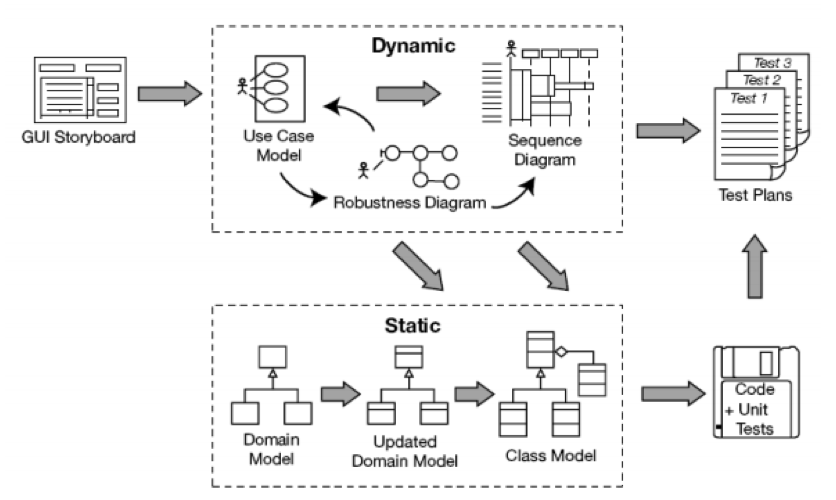
\includegraphics[scale=0.95]{./imagens/visao_geral_iconix.png}}
	\caption[Uma visão geral do ICONIX e seus componentes.]
	{Uma visão geral do ICONIX e seus componentes. \textbf{Fonte:} \citeonline{rosenberg_scott_use_case_driven_object_modeling_with_uml}}
	\label{fig:visao_geral_iconix_componentes}
\end{figure}

\newpage %Pular pagina para que o texto fica abaixo da imagem na nova pagina

\par Ao utilizar essa metodologia, o desenvolvimento do projeto passa a ser norteado por casos de uso (\textit{use cases}) e suas principais fases são: análise de requisitos, análise e projeto preliminar, projeto e implementação. A seguir será apresentada uma breve descrição de cada uma das fases do ICONIX, seguindo as ideias de \citeonline{o_engenheiro_software_as_fases_iconix_mecva}.

\subsection{Análise de requisitos}

A função da fase de análise de requisitos é modelar os objetos do problema real a partir dos requisitos do software já levantados, e, a partir destes objetos gerar o diagrama de modelo de domínio. Ainda nesta fase, e, com base nos requisitos, deve-se definir os casos de uso do \textit{software}. Estes casos de uso são o elo entre os requisitos e a implementação propriamente dita do \textit{software}. Por isto, a definição destes diagramas se faz tão importante para o ICONIX. 

%A fase de análise de requisitos tem como finalidade identificar os objetos do problema real e, a partir destes objetos definir como eles serão abstraídos para o software por meio do modelo de domínio. Estes objetos são identificados a partir dos requisitos que foram levantados anteriormente. Também apresenta um protótipo das possíveis interfaces gráficas e, por fim, descrever os casos de uso. Quando possível, elabora-se os diagramas de navegação para que o cliente possa entender melhor o funcionamento do sistema como um todo.

\subsection{Análise e projeto preliminar}

Nesta fase deve-se detalhar todos os casos de uso identificados na fase de análise de requisitos, por meio de diagramas de robustez, baseando-se no texto dos casos de uso (fluxo de eventos). O diagrama de robustez não faz parte dos diagramas padrões da UML. Porém, este é utilizado para descobrir as classes de análise e detalhar superficialmente o funcionamento dos casos de uso.

Em paralelo, deve-se atualizar o modelo de domínio adicionando os atributos identificados às suas respectivas entidades, que foram descobertas na fase de análise de requisitos. A partir deste momento será possível gerar a base de dados do sistema.


\subsection{Projeto detalhado}

\par Na fase denominada projeto detalhado deve-se elaborar o diagrama de sequência com base nos diagramas de casos de uso identificados anteriormente, a fim de detalhar sua implementação.

O diagrama de sequência deve conter as classes que serão implementadas e as mensagens enviadas entre os objetos corresponderão às operações que realmente serão implementadas futuramente. Estas operações devem ser incluídas no modelo de domínio em conjunto com as novas classes do projeto identificadas, criando assim, o diagrama de classes final.

\subsection{Implementação}

Na fase de implementação deve-se desenvolver o código fonte do \textit{software} e os testes necessários para obter um software com qualidade. O ICONIX não define os passos a serem seguidos nesta fase, ficando a cargo de cada um definir a forma como será implementado o projeto.
 
Ao término de cada fase um artefato é gerado, sendo respectivamente: revisão dos requisitos, revisão do projeto preliminar, revisão detalhada e entrega.

O ICONIX é considerado um processo prático de desenvolvimento de software, pois a partir das iterações que ocorrem na análise de requisitos e na construção dos modelos de domínios (parte dinâmica), os diagramas de classes (parte estática) são incrementados e, a partir destes, o sistema poderá ser codificado.


Por proporcionar essa praticidade, o ICONIX será empregado para o desenvolvimento deste projeto, pois por meio dele é possível obter produtividade no desenvolvimento do \textit{software} ao mesmo tempo em que alguns artefatos são gerados, unindo o aspecto de abrangência e agilidade.
